\documentclass[11pt]{article}

\usepackage{graphicx}
\usepackage{amsmath}
\usepackage{mathtools}
\usepackage{amssymb}
\usepackage[T1]{fontenc}
\usepackage[lithuanian]{babel}
\usepackage{listings}
\usepackage{subfigure}

\topmargin=-0.45in
\evensidemargin=0in
\oddsidemargin=0in
\textwidth=6.5in
\textheight=9.0in
\headsep=0.25in
    
\title{ Antras laboratorinis darbas}
\author{ Arnas Vaicekauskas }
\date{\today}

\begin{document}
\maketitle

\section{Uždavinys}

Išspręsti pirmos eilės diferencialinę lygtį su Koši pradine sąlyga naudojanti Rungės-Kuto 3-pakopį ir 4-pakopį skaitinius modelius.

\begin{align}
u'&=x+2x^2\sin(u)\\
u(0)&=-1
\end{align}

\section{Skaitiniai modeliai}

Skaitiniai modeliai įgyvendinti naudojant python programavimo kalbą, numpy ir scipy paketus.

\subsection{Rungė-Kuto 3-pakopis modelis}

\begin{align}
    \begin{cases}
        k_1&=f(x_n,y_n)\\
        k_2&=f(x_n+\tau,y_n+\tau k_1)\\
        k_3&=f(x_n+\frac{\tau}{2},y_n+\frac{\tau}{2}\frac{k_1+k_2}{2})\\
    \end{cases}\\
    y_{n+1}=y_n+\frac{\tau}{6}(k_1+k_2+4k_3).
\end{align}

\subsection{Rungė-Kuto 4-pakopis modelis}

\begin{align}
    \begin{cases}
        k_1&=f(x_n,y_n)\\
        k_2&=f(x_n+\frac{\tau}{2},y_n+\frac{\tau}{2}k_1)\\
        k_3&=f(x_n+\frac{\tau}{2},y_n+\frac{\tau}{2}k_2)\\
        k_4&=f(x_n+\tau,y_n+\tau k_3)\\
    \end{cases}\\
    y_{n+1}=y_n+\frac{\tau}{6}(k_1+2k_2+2k_3+k_4).
\end{align}

\newpage
\section{Rezultatai}

\subsection{Žymėjimas}

$x$ - laisvas kintamasis, 
$u_\tau$ - skaitinis sprendinys su žingsniu $\tau$,
$u_\tau(x)$ - skaitinio sprendinio su žingsniu $\tau$ reikšmė koordinatėje $x$,
$u(x)$ - analitinio sprendinio reikšmė koordinatėje $x$.

\subsection{Sprendinių grafikai}

\subsubsection{(a) dalis}

\begin{figure}[h!]
    \centering
    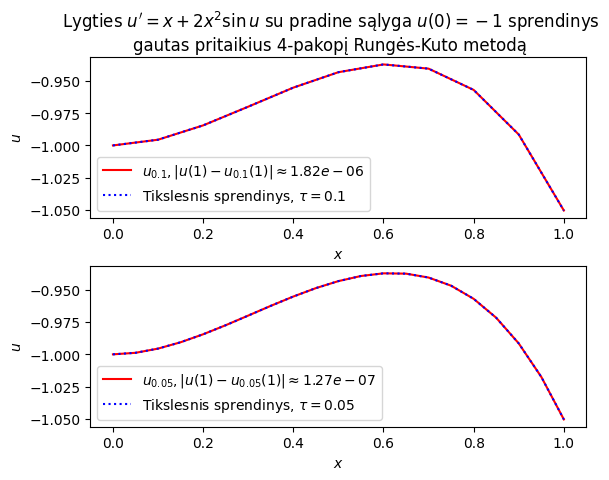
\includegraphics[width=0.8\textwidth]{a1.png}
    \caption{Skaitiniai lygties sprendiniai, kai $\tau=0.1, 0.05$ lyginami su tikslesniu sprendiniu gautu naudojant scipy metodą odeint.}
    \label{fig:pvz1}
\end{figure}

\newpage
\subsubsection{(b) dalis}

\begin{figure}[h!]
    \centering
    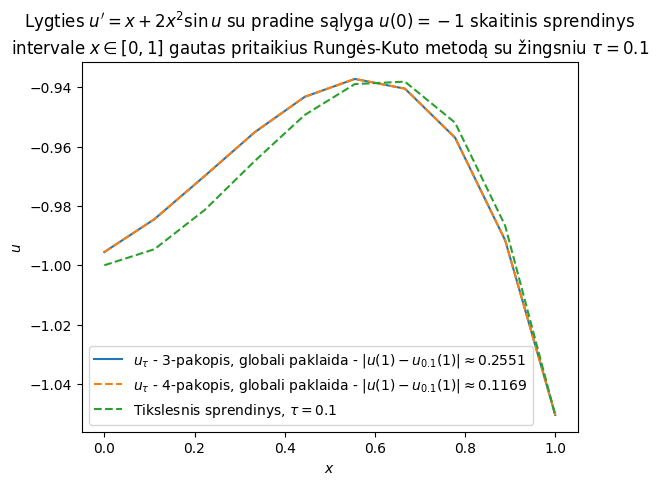
\includegraphics[width=0.8\textwidth]{b1.png}
    \caption{Skaitiniai lygties sprendiniai gauti skirtingais metodais lyginami su tikslesniu sprendiniu gautu naudojant scipy metodą odeint.}
    \label{fig:pvz2}
\end{figure}

\newpage
\subsection{Paklaidos vertinimas}

Rungės metodas paklaidai įvertinti

\begin{align}
\vert u(x)-u_{\tau}(x)\vert\approx\frac{\vert u_{2\tau}(x) - u_{\tau}(x)\vert}{2^p - 1}
\end{align}

\begin{figure}[h!]
    \centering
    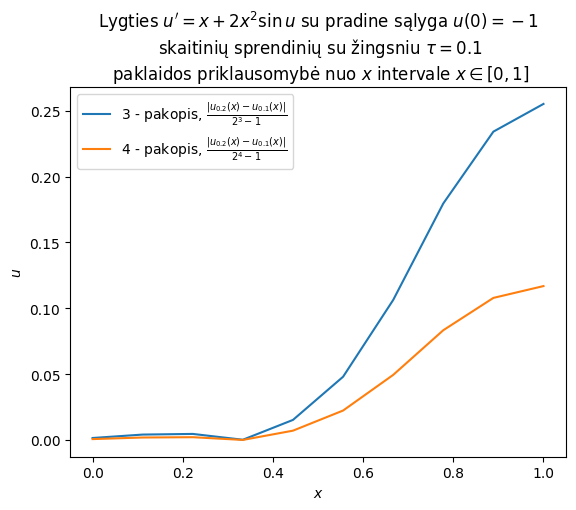
\includegraphics[width=0.8\textwidth]{error.png}
    \caption{Skaitinių metodų paklaidos.}
    \label{fig:pvz3}
\end{figure}

\newpage
\section{Priedai}

Programos kodas naudotas sugeneruoti visus šiame dokumente esančius grafikus.

\subsection{solver.py}

\begin{lstlisting}[language=Python]
import numpy as np

def rk3(f, t_0, y_0, tau, N):
    ts = np.linspace(t_0, t_0 + (N - 1) * tau, N)
    ys = np.zeros(N)
    ys[0] = y_0
    for i in range(N - 1):
        k1 = f(ts[i], ys[i])
        k2 = f(ts[i] + tau, ys[i] + tau * k1)
        k3 = f(ts[i] + tau/2, ys[i] + tau/2 * (k1 + k2)/2 )
        ys[i + 1] = ys[i] + tau/6 * (k1 + k2 + 4*k3)
    return ts, ys

def rk4(f, t_0, y_0, tau, N):
    ts = np.linspace(t_0, t_0 + (N - 1) * tau, N)
    ys = np.zeros(N)
    ys[0] = y_0
    for i in range(N - 1):
        k1 = f(ts[i], ys[i])
        k2 = f(ts[i] + tau/2, ys[i] + tau/2 * k1)
        k3 = f(ts[i] + tau/2, ys[i] + tau/2 * k2)
        k4 = f(ts[i] + tau, ys[i] + tau * k3)
        ys[i + 1] = ys[i] + tau/6 * (k1 + 2*k2 + 2*k3 + k4)
    return ts, ys
\end{lstlisting}

\newpage
\subsection{different-steps.py}

\begin{lstlisting}[language=Python]
import numpy as np
from scipy.integrate import odeint
import matplotlib.pyplot as plt
from solver import rk3, rk4

def f(t, u):
    return t + 2 * t ** 2 * np.sin(u)

u_0 = -1
x_0 = 0
x_end = 1

fig, axes = plt.subplots(2, sharey=True)

fig.suptitle("")

plt.xlabel("")
plt.ylabel("")

for index, tau in enumerate([0.1, 0.05]):

    N = int((x_end - x_0) / tau) + 1
    M = int((x_end - x_0) / (2 * tau)) + 1

    xs, us = rk4(f, x_0, u_0, tau, N)

    _, us_2tau = rk4(f, x_0, u_0, 2 * tau, M)
    error = np.abs(us_2tau[-1] - us[-1]) / (2**4 - 1)
    axes[index].plot(xs, us, label="", color='red')

    us_real = odeint(f, u_0, xs, tfirst=True)
    axes[index].plot(xs, us_real,label="", linestyle='dotted', color='blue')

    axes[index].set_xlim((-0.05, x_end+0.05))

    axes[index].legend()

fig.subplots_adjust(wspace=0.2)

plt.show()
\end{lstlisting}

\newpage
\subsection{different-method.py}

\begin{lstlisting}[language=Python]
import numpy as np
from scipy.integrate import odeint
import matplotlib.pyplot as plt
from solver import rk3, rk4

def f(t, u):
    return t + 2 * t ** 2 * np.sin(u)

u_0 = -1
x_0 = 0
x_end = 1
tau = 0.05

plt.title("")

plt.xlabel("")
plt.ylabel("")

N = int((x_end - x_0) / tau) + 1
M = int((x_end - x_0) / (2 * tau)) + 1

xs, us_3 = rk3(f, x_0, u_0, tau, N)

us_real = odeint(f, u_0, xs, tfirst=True)
plt.plot(xs, us_real,label="", linewidth=4, color='green')

_, us_3_2tau = rk3(f, x_0, u_0, 2 * tau, M)
error_3_global = np.abs(us_3_2tau[-1] - us_3[-1]) / (2**3 - 1)
plt.plot(xs, us_3, label="", marker='D', color='red')

_, us_4 = rk4(f, x_0, u_0, tau, N)
_, us_4_2tau = rk4(f, x_0, u_0, 2 * tau, M)
error_4_global = np.abs(us_4_2tau[-1] - us_4[-1]) / (2**4 - 1)
plt.plot(xs, us_4, label="", marker='x', color='yellow')

plt.gca().set_xlim((-0.05, x_end+0.05))

plt.legend()
plt.show()
\end{lstlisting}

\newpage
\subsection{error.py}

\begin{lstlisting}[language=Python]
import numpy as np
from scipy.integrate import odeint
import matplotlib.pyplot as plt
from solver import rk3, rk4

def f(t, u):
    return t + 2 * t ** 2 * np.sin(u)

u_0 = -1
x_0 = 0
x_end = 1
tau = 0.05

N = int((x_end - x_0) / tau) + 1
M = int((x_end - x_0) / (2 * tau)) + 1

_, us_3 = rk3(f, x_0, u_0, tau, N)
xs, us_3_2tau = rk3(f, x_0, u_0, 2 * tau, M)

_, us_4 = rk4(f, x_0, u_0, tau, N)
_, us_4_2tau = rk4(f, x_0, u_0, 2 * tau, M)

error_rk3 = np.abs(us_3_2tau - us_3[::2]) / (2**3 - 1)
error_rk4 = np.abs(us_4_2tau - us_4[::2]) / (2**4 - 1)

plt.title("")

plt.plot(xs, error_rk3, label="")
plt.plot(xs, error_rk4, label="")
plt.legend()
plt.xlabel("")
plt.ylabel("")

plt.gca().set_ylim((0, 0.00001))
plt.gca().set_xlim((-0.05, x_end+0.05))

plt.show()
\end{lstlisting}

\end{document}